

\chapter{Modelling and Analysis of Collaborative Node Kinematic Behaviuors in Underwater Acoustic MANETs} % Write in your own chapter title
\label{Chapter\thechapter}
\lhead{Chapter \thechapter. \emph{\nameref{Chapter\thechapter}}} % Write in your own chapter title to set the page header



\subsection{Establishing Scale Factors in Communications Rate}

In this section we characterise the simulated communications environment, establishing an optimal packet emission rate for comparison against \cite{Guo11}.

In order to establish the point at which the network becomes saturated due, a range of packet emission rates were explored between 0.01 packets per second (pps), equivalent to 96 bps, up to 0.07 pps (672 bps)

From Figs.~\ref{fig:throughput_performance_static} and ~\ref{fig:prod_breakdown_static}, it is clear that the threshold curve, expressed as the \emph{Successfully Received Packets} line, exhibits a saturation point between 0.025 and 0.03 pps.
Particularly in Fig.~\ref{fig:prod_breakdown_static}, the precipitous drop in packet delivery probability beyond 0.025 pps, indicating that this is a strong candidate value for an upper-limit to the safe operating zone in terms of packet emission in the small static case.

\begin{figure}[H]
  \centering
  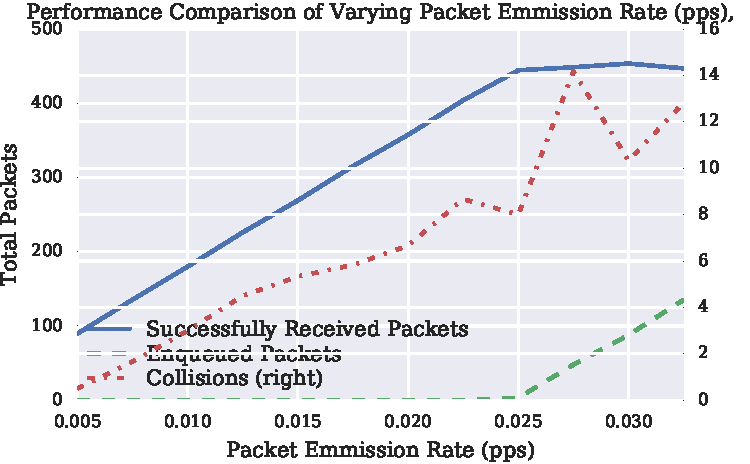
\includegraphics[width=0.6\textwidth]{img/throughput_performance_static.pdf}
  \caption{Varying packet emission rate demonstrates maximal throughput at 0.025 packets per second, equivalent to $\approx$240 bps}
  \label{fig:throughput_performance_static}
\end{figure}


\begin{figure}[H]
  \centering
  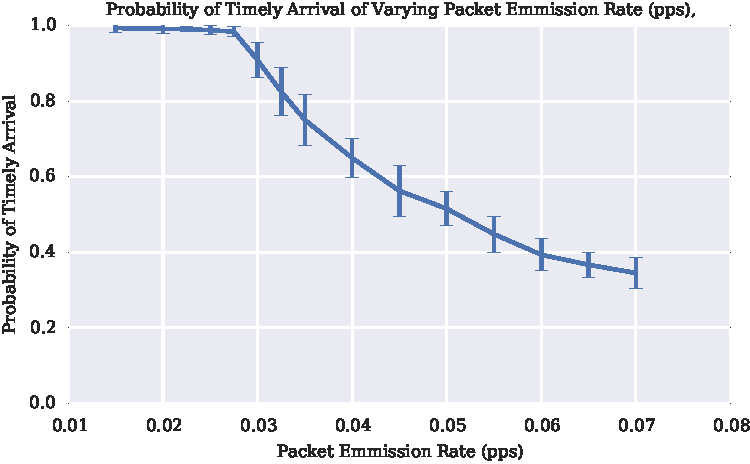
\includegraphics[width=0.6\textwidth]{img/prod_breakdown_static.pdf}
  \caption{Varying packet emission rate demonstrates a saturation point at 0.025 packets per second}
  \label{fig:prod_breakdown_static}
\end{figure}

\subsection{Establishing Scale Factors in Physical Distribution}

In this section we characterise the effect of node-separation scaling on communications operation for comparison against \cite{Guo11}. This is particularly important considering the significant scale factor differences between not only the speed of propagation in the medium, but simply the range of operation. 
From Table \ref{tab:sysconstraints}, the operating transmission range of acoustic is $\approx 6$ times further than 802.11, indicating that a suitable operating environment will have an area $\approx \sqrt{6}$ times the area of the 802.11 case. Therefore, a reasonable experimental range would have an upper bound of performance around this scaling factor, where nodes are approximately 400$m$ apart. 

A reasonable range around this is to scale from 100$m$ apart on average to 800$m$.

Varying average node separation shows that while direct throughput isn't significantly affected until, collision rates are Fig.~\ref{fig:throughput_performance_range}.
This collision rate is well within the tolerances of the MAC layer, as shown in Fig.~\ref{fig:prod_breakdown_range}, where even with a rising collision rate, packets are being reliably received.

\begin{figure}[H]
  \centering
  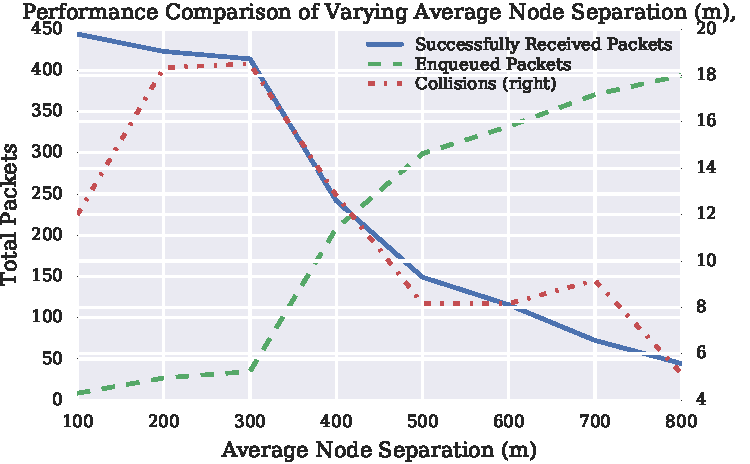
\includegraphics[width=0.6\textwidth]{img/throughput_performance_range.pdf}
  \caption{Comparison of Medium Acquisition Collisions, Throughput, and Enqueued packets against varying application packet emission rates.}
  \label{fig:throughput_performance_range}
\end{figure}

\begin{figure}[H]
  \centering
  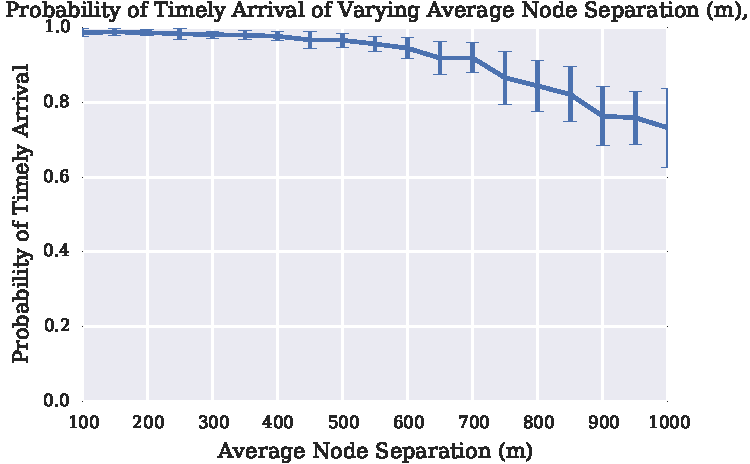
\includegraphics[width=0.6\textwidth]{img/prod_breakdown_range.pdf}
  \caption{Probability of Timely Reception across a range of node scaling.}
  \label{fig:prod_breakdown_range}
\end{figure}

However, when end-to-end delay is investigated, it's clear from Fig.~\ref{fig:delay_range} that the network is becoming severely impaired approaching the 600$m$ mark, with delays rising to more than 25 minutes above 700$m$.
This is also demonstrated by the increasing RTS/Data ratio shown in Fig.~\ref{fig:rts_range}.

According to Xu \cite{Xu2002}, the RTS/CTS handshake cannot function well as interference protection at node separations beyond 0.56 times the transmission range. 
This is also demonstrated in  Fig.~\ref{fig:rts_range}, where above $1500m \times 0.56 = 840m$, 
This is due to reduced channel availability due to collisions, which are then due to a much longer potential contention period between nodes. 

\begin{figure}[H]
  \centering
  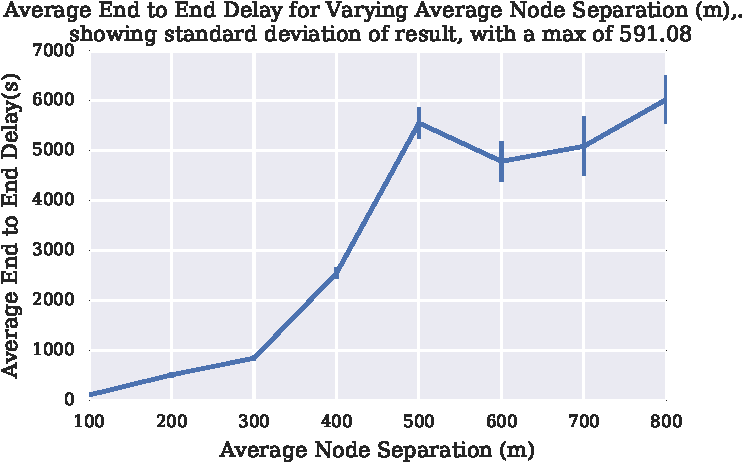
\includegraphics[width=0.6\textwidth]{img/delay_range.pdf}
  \caption{End to End Delay under varying node-separations}
  \label{fig:delay_range}
\end{figure}

\begin{figure}[H]
  \centering
  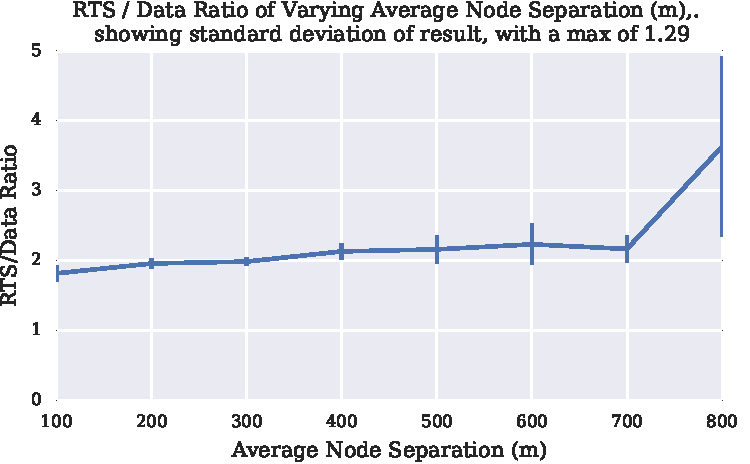
\includegraphics[width=0.6\textwidth]{img/rts_range.pdf}
  \caption{RTS/Data ratio for varying node-separations}
  \label{fig:rts_range}
\end{figure}


\begin{table}[H]
  \caption{Tabular view of data from Figs~\ref{fig:prod_breakdown_range}, \ref{fig:delay_range}, and \ref{fig:rts_range}} \label{tab:rangedelay}
  \begin{center}
      \hyphenpenalty 100000
      \begin{tabular}{
*{2}{@{\hspace{1em}}r@{\hspace{1em}}}
*{3}{@{\hspace{1em}}p{0.1\textwidth} @{\hspace{1em}}}  }
\toprule
 Separation(m) &  Delay(s) &  Probability of Arrival &  RTS/Data Ratio &  Ideal Delivery Time(s) \\
\midrule
           100 &     60.32 &                    0.99 &            1.80 &                    1.03 \\
           200 &    419.95 &                    0.97 &            2.02 &                    1.10 \\
           300 &   1205.66 &                    0.89 &            2.41 &                    1.17 \\
           400 &   1288.20 &                    0.91 &            2.26 &                    1.25 \\
           500 &   1868.20 &                    0.87 &            2.41 &                    1.32 \\
           600 &   2191.07 &                    0.85 &            2.42 &                    1.39 \\
\bottomrule
\end{tabular}

  \end{center}
\end{table}



\subsection{Metric Weighting}
\begin{figure}
\begin{subfigure}{.5\textwidth}
  \centering
  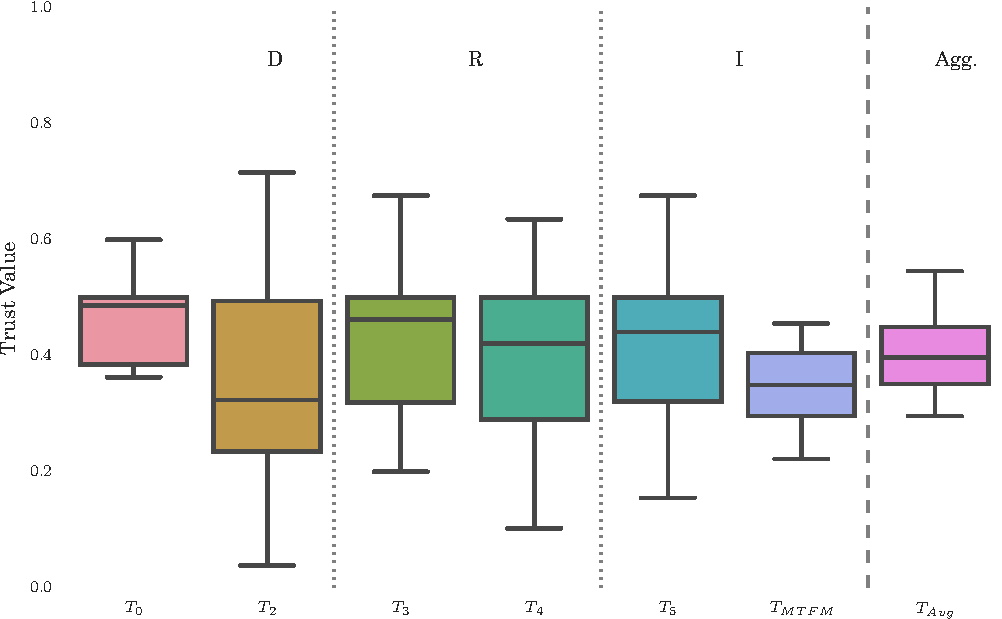
\includegraphics[width=.95\linewidth]{img/trust_bella_static_selfish.pdf}
  \caption{All Nodes Static}
  \label{fig:selfish_trust_static}
\end{subfigure}%
\begin{subfigure}{.5\textwidth}
  \centering
  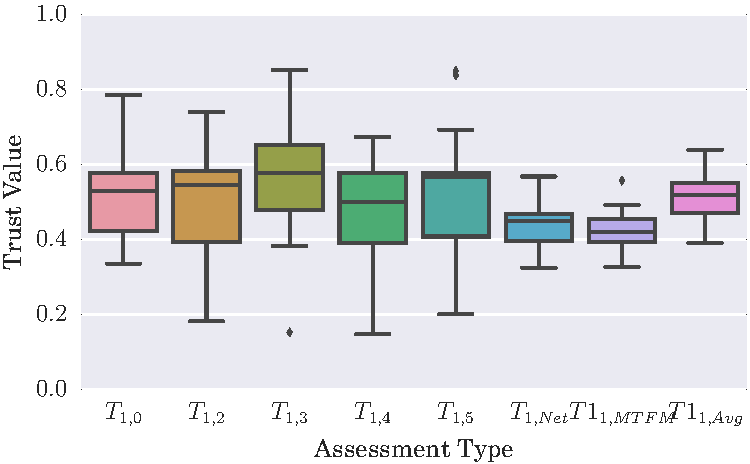
\includegraphics[width=.95\linewidth]{img/trust_bella_single_mobile_selfish.pdf}
  \caption{$n_1$ Randomly Walking}
  \label{fig:selfish_trust_single}
\end{subfigure}
\begin{subfigure}{.5\textwidth}
\centering
  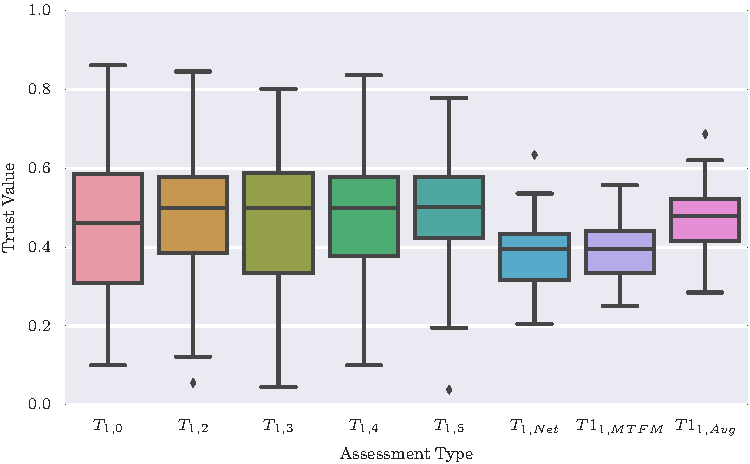
\includegraphics[width=.95\linewidth]{img/trust_bella_allbut1_mobile_selfish.pdf}
  \caption{All Nodes but $n_1$ Randomly Walking}
  \label{fig:selfish_trust_allbut1}
\end{subfigure}
\begin{subfigure}{.5\textwidth}
\centering
  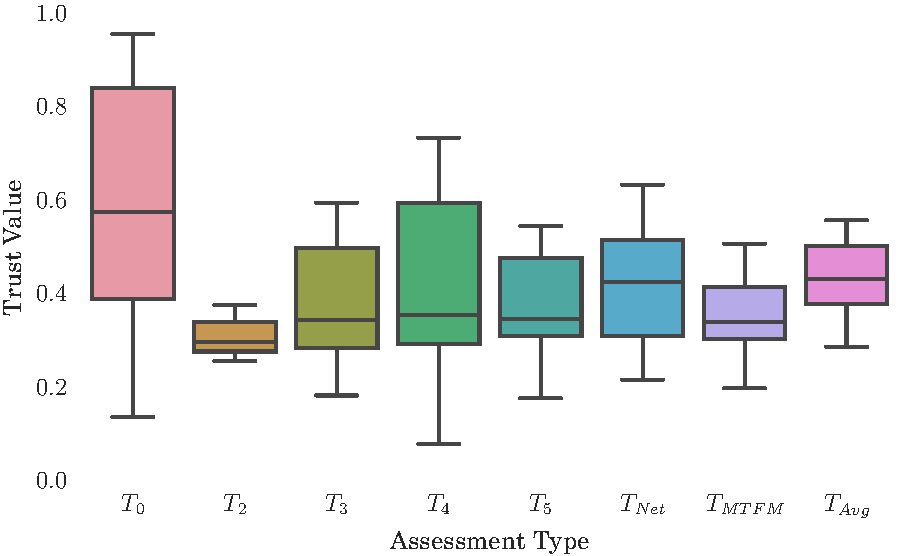
\includegraphics[width=.95\linewidth]{img/trust_bella_all_mobile_selfish.pdf}
  \caption{All Nodes Randomly Walking}
  \label{fig:selfish_trust_all_mobile}
\end{subfigure}
\caption{MTFM Trust assessments for varying mobility options in the selfish case}
\label{fig:trust_mobility}
\end{figure}



\begin{figure}
\begin{subfigure}{\textwidth}
  \centering
  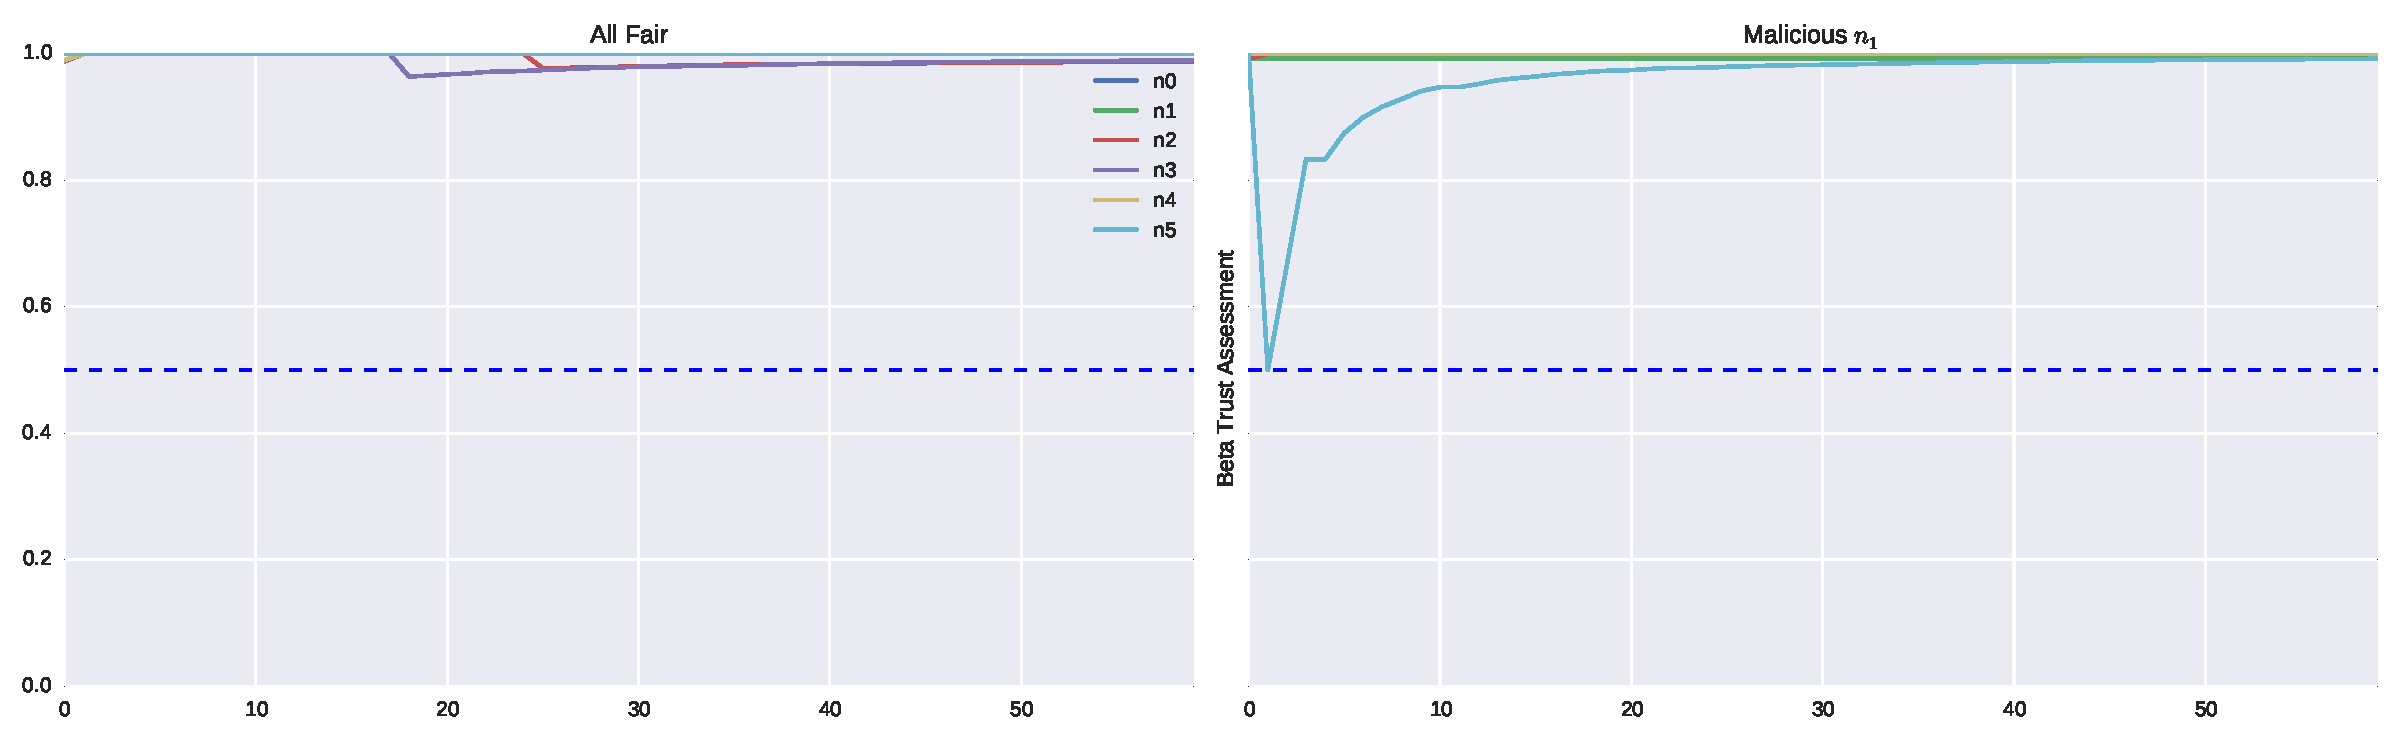
\includegraphics[width=.95\linewidth]{img/beta_trust_bella_static_joint.pdf}
  \caption{All Nodes Static}
  \label{fig:beta_trust_static}
\end{subfigure}
\begin{subfigure}{\textwidth}
  \centering
  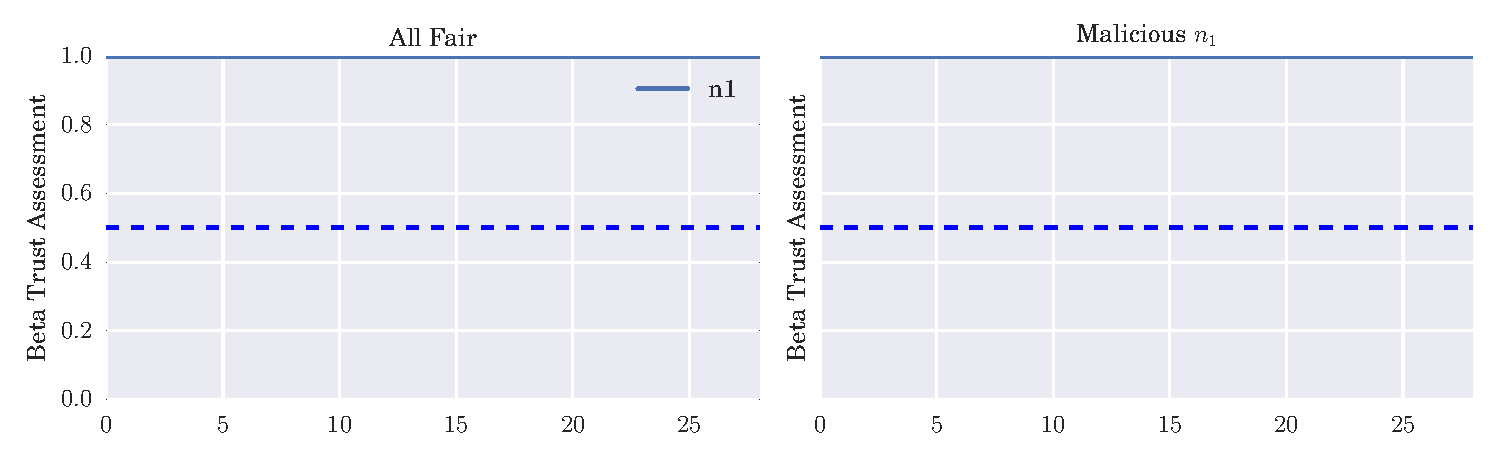
\includegraphics[width=.95\linewidth]{img/beta_trust_bella_single_mobile_joint.pdf}
  \caption{$n_1$ Randomly Walking}
  \label{fig:beta_trust_single}
\end{subfigure}
\begin{subfigure}{\textwidth}
\centering
  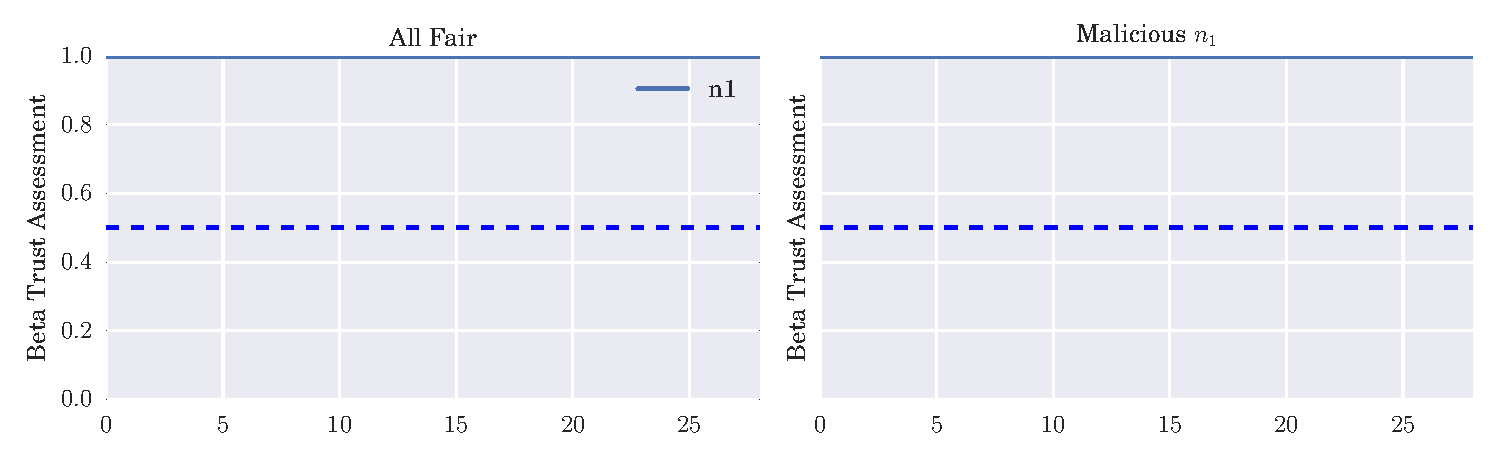
\includegraphics[width=.95\linewidth]{img/beta_trust_bella_allbut1_mobile_joint.pdf}
  \caption{All Nodes but $n_1$ Randomly Walking}
  \label{fig:beta_trust_allbut1}
\end{subfigure}
\begin{subfigure}{\textwidth}
\centering
  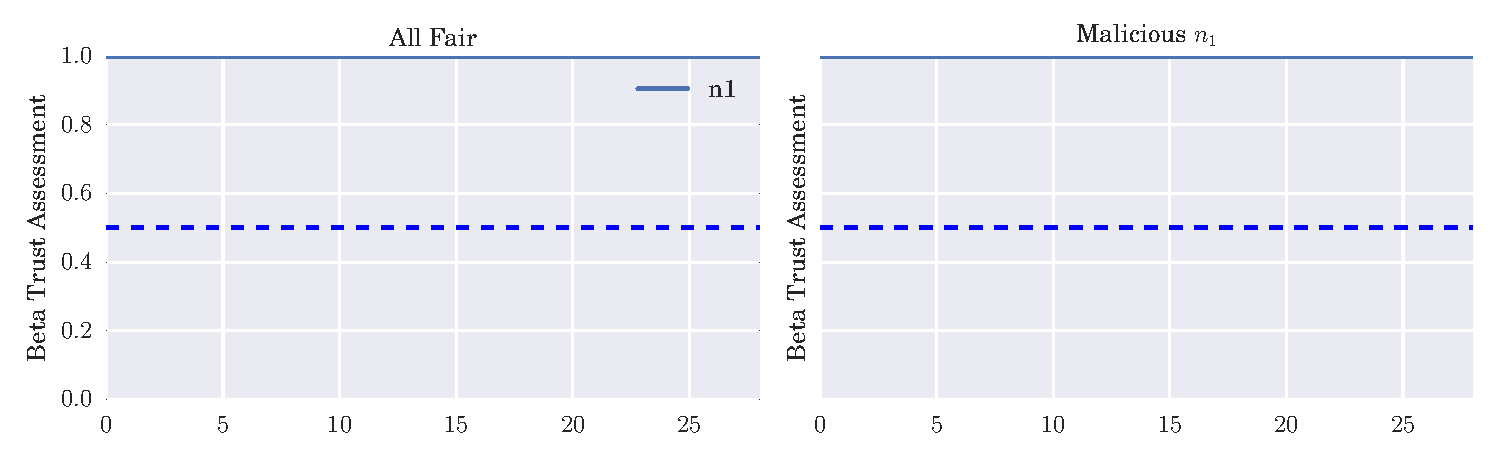
\includegraphics[width=.95\linewidth]{img/beta_trust_bella_all_mobile_joint.pdf}
  \caption{All Nodes Randomly Walking}
  \label{fig:beta_trust_all_mobile}
\end{subfigure}
\caption{Beta Trust time varying assessments for of $n1$ varying mobility options}
\label{fig:trust_mobility}
\end{figure}



